 \TChapter{Avances}{epsilon}
\ \\\\
En esta sección se mostrarán los avances que hasta el día de hoy se tienen.

%-----------------------------------------------------------------------------------------%
\section{Herramientas utilizadas}
Para el desarrollo de los avances en el presente trabajo, se utilizó el lenguaje de programación Python\footnote{https://www.python.org/} 
en la distribución Anaconda\footnote{https://www.anaconda.com/distribution/}, ya que gestiona las 
versiones de las librerías utilizadas para el análisis de datos, y para el recolector web (Crawler) se utilizó Scrapy\footnote{https://scrapy.org/}, 
un framework que permite la extracción de información de sitios web.

%-----------------------------------------------------------------------------------------%

\section{Estudio previo}
Una vez elegidas las herramientas que permiten la extracción de la información, se procedió con la selección de los 
sitios web para extraer noticias.
\\
El sitio web El Economista\footnote{https://www.eleconomista.com.mx/} contiene una sección llamada 
\textbf{Ranking de Medios Nativos Digitales}\footnote{https://www.eleconomista.com.mx/Ranking-de-Medios-Nativos-Digitales}, 
el cual muestra las estadísticas que realiza mes con mes acerca de los sitios de noticias web más consultados como se muestra 
en la Figura \textbf{\ref{fig:rank}}
\begin{figure}[H]
  \centering
  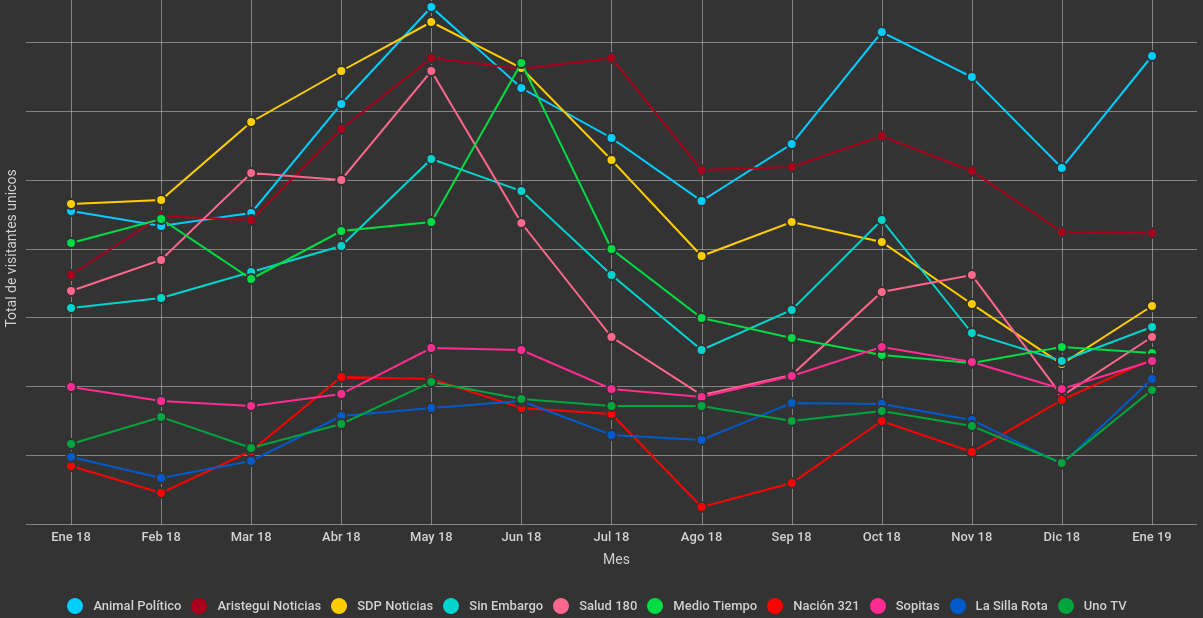
\includegraphics[scale=.28]{imagenes/Capitulo5/ranking}
  \caption{Ranking de sitios de noticias del periódo de enero del 2018 a enero del 2019.}
  \label{fig:rank}
\end{figure}
 

Para la selección final de los sitios de noticias que se utilizarán en estre trabajo, se revisaron los los medios mostrados en la Figura 5.1. Después de esta revisión se encontró que los sitios Salud 180 y Medio Tiempo muestran noticias relacionadas únicamente con salud y deportes respectivamente. En este trabajo se desean obtener noticias de diversas secciones por lo que estos sitios se descartaron. También para este trabajo es importante incluir información de otros medios como diarios y  sitios de televisón, por lo tanto se incluyeron sitios relacionados con estos medios.

\begin{itemize}
    \item 3 Sitios de foros de noticias: 
    \begin{itemize}
      \item \textbf{Aristegui Noticias}: https://aristeguinoticias.com/
      \item \textbf{SDP Noticias}: https://www.sdpnoticias.com/
      \item \textbf{Sopitas}: https://www.sopitas.com/
    \end{itemize}
    \item 3 Sitios de diarios:
    \begin{itemize}
      \item \textbf{El Universal}: https://www.eluniversal.com.mx/
      \item \textbf{La Jornada}: https://www.jornada.com.mx/
      \item \textbf{Exélsior}: https://www.excelsior.com.mx/
    \end{itemize}
    \item 3 Sitios de televisión:
    \begin{itemize}
      \item \textbf{TV Azteca}: https://www.aztecanoticias.com.mx/
      \item \textbf{Televisa}: https://noticieros.televisa.com/
      \item \textbf{Once Noticias}: https://www.oncenoticias.tv/
    \end{itemize}
\end{itemize}

Los sitios organizan las noticias en secciones. Una vez seleccionados los sitios, se procedió con el análisis de las secciones que contienen los portales, como 
lo muestra la Tabla \textbf{\ref{tabla:sitios}}.

\begin{table}[htbp]
    \centering
    \resizebox{\columnwidth}{!}{%
    \begin{tabular}[H]{|l|l|l|l|l|l|l|l|l|}


 \multicolumn{1}{| >{\columncolor{myBlueChapter}}l|}{ \textcolor{myWhite}{\textbf{El}} }
&\multicolumn{1}{| >{\columncolor{myBlueChapter}}l|}{ \textcolor{myWhite}{\textbf{La}} }
&\multicolumn{1}{| >{\columncolor{myBlueChapter}}l|}{ \textcolor{myWhite}{\textbf{Milenio}} }
&\multicolumn{1}{| >{\columncolor{myBlueChapter}}l|}{ \textcolor{myWhite}{\textbf{Aristegui}} }
&\multicolumn{1}{| >{\columncolor{myBlueChapter}}l|}{ \textcolor{myWhite}{\textbf{SDP}} }
&\multicolumn{1}{| >{\columncolor{myBlueChapter}}l|}{ \textcolor{myWhite}{\textbf{Sopitas}} }
&\multicolumn{1}{| >{\columncolor{myBlueChapter}}l|}{ \textcolor{myWhite}{\textbf{Azteca}} }
&\multicolumn{1}{| >{\columncolor{myBlueChapter}}l|}{ \textcolor{myWhite}{\textbf{Televisa}} }
&\multicolumn{1}{| >{\columncolor{myBlueChapter}}l|}{ \textcolor{myWhite}{\textbf{Once}} }
  \\ \cline{1-9}
%---------------------------------------------------------------------------------------%

 \multicolumn{1}{| >{\columncolor{myBlueChapter}}l|}{ \textcolor{myWhite}{\textbf{Universal}} }
&\multicolumn{1}{| >{\columncolor{myBlueChapter}}l|}{ \textcolor{myWhite}{\textbf{Jornada}} }
&\multicolumn{1}{| >{\columncolor{myBlueChapter}}l|}{ }
&\multicolumn{1}{| >{\columncolor{myBlueChapter}}l|}{ \textcolor{myWhite}{\textbf{Noticias}} }
&\multicolumn{1}{| >{\columncolor{myBlueChapter}}l|}{ \textcolor{myWhite}{\textbf{Noticias}} }
&\multicolumn{1}{| >{\columncolor{myBlueChapter}}l|}{ }
&\multicolumn{1}{| >{\columncolor{myBlueChapter}}l|}{ \textcolor{myWhite}{\textbf{Noticias}} }
&\multicolumn{1}{| >{\columncolor{myBlueChapter}}l|}{ }
&\multicolumn{1}{| >{\columncolor{myBlueChapter}}l|}{ \textcolor{myWhite}{\textbf{Noticias}} }
\\ \cline{1-9}

%---------------------------------------------------------------------------------------%

        Nacional      & -            & Nacional      & México                & Nacional      & Noticias  & -                 & Nacional      & Nacional      \\ 
        \hline
%---------------------------------------------------------------------------------------%

       	Mundo         & Mundo        & Mundo         & Destacado o       & Internacional & -         & Internacional     & Internacional & Internacional \\ 
        & & & Mundo & & & & & \\ 
        \hline
%---------------------------------------------------------------------------------------%

        Metrópoli     & Capital      & CDMX          & -                     & -             & -         & -                 & CDMX          & CDMX      \\ 
        \hline
%---------------------------------------------------------------------------------------%

        Estados       & Estados      & Estados       & Sociedad o       & Estados       & -         & Estados           & Estados       & Nacional   \\ 
        & & & México & & & & & \\ 
        \hline
%---------------------------------------------------------------------------------------%

        Cartera       & Economía     & Negocios      & Economía              & Economía      & -         & Finanzas          & Economía      & Economía   \\ 
        \hline
%---------------------------------------------------------------------------------------%

        Deportes      & Deportes     & La Afición    & Deportes              & Deportes      & Deportes  & -                 & Deportes      & Deportes   \\ 
        \hline
%---------------------------------------------------------------------------------------%

        Espectáculos  & Espectáculos & Hey           & -                     & En el show    & Entretenimiento & -           & Entretenimiento & Deportes    \\ 
        \hline
%---------------------------------------------------------------------------------------%

        Cultura       & Cultura      & Cultura       & -                     & -             & -         & -                 & Arte y cultura & Cultura   \\ 
        \hline
%---------------------------------------------------------------------------------------%

        Nación o & Política   & Política      & Poderes               & -             & -         & Política          & Política      & -   \\ 
        & política & & & & & & & \\ 
        \hline
%---------------------------------------------------------------------------------------%

        Ciencia y & Tecnología & Tecnología    &                       & Geek          & Geek      & -                 & Tecnología*      & Ciencia\\
        salud & & & & & & & & \\ 
        \hline        

    \end{tabular}%
}
\caption[Tabla]{Secciones existentes en los sitios web}
\label{tabla:sitios}
\end{table}

Una vez que se analizarón las secciones con las que contaba cada sitio se procedió a homologar las secciones en las cuales la mayoría de los sitios coincidian, por lo cual se quedarón definidas 5 secciones para clasificación de las noticia:

\begin{itemize}
    \item Política
    \item Deportes
    \item Ciencia y tecnología
    \item Economía
    \item Cultura
\end{itemize}

Para llevar a cabo el proceso de extracción de las noticias, se realizó el estudio 
de la estructura XML (\textit{Extensible Markup Language}), por sus siglas en inglés de cada sitio web seleccionado, con 
el objetivo de definir las etiquetas que poseen la información de las noticias, las cuales son:

\begin{itemize}
  \item URL
  \item Sección
  \item Título
  \item Autor
  \item Fecha
  \item Descripción
  \item Noticia
\end{itemize} 

%-----------------------------------------------------------------------------------------%
\section{Recolección de noticias}
En la siguiente Figura \textbf{\ref{fig:diagrama}}. se describe el proceso de recolección:

\begin{figure}[H]
  \centering
  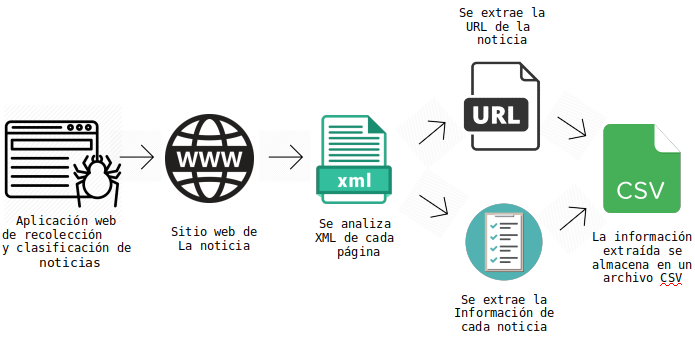
\includegraphics[scale=.50]{imagenes/Capitulo5/diagrama}
  \caption{Proceso de recolección de noticias.}
  \label{fig:diagrama}
\end{figure}

%-----------------------------------------------------------------------------------------%
\subsection{Desarrollo}

Con base en la información obtenida de los sitios web, se diseño un recolector de noticias para cada sitio, procede con 
los siguientes pasos para realizar la extracción de noticias.

\begin{itemize}
  \item Se ingresa a la URL definida como inicio y se analiza la etiqueta definida que redirecciona a cada noticia del sitio web
  \item Una vez que se ha ingresado a la noticia se procede con el análisis de las etiquetas definidas
  \item Se extrae la información de cada noticia, así como su URL
  \item Posteriormente la información recolectada se guarda en un archivo csv
\end{itemize}
La siguiente figura muestra el comando que realiza el proceso de recolección de las noticias.

%Para el proceso de extracción se abre una terminal con la ruta donde se guardará la información recolectada Figura \textbf{\ref{fig:uno}} 
%Se va a redactar los pasos del proceso de recolección

%-----------------------------------------------------------------------------------------%
\subsection{Resultados}

%-----------------------------------------------------------------------------------------%
\subsubsection{Secciones recolectadas}

De los nueve sitios web definidos se obtuvieros las siguientes secciones mostrados en la Tabla \textbf{\ref{tabla:secciones}}:
\\
\begin{table}[htbp]
  \centering
  \resizebox{\columnwidth}{!}{%
  \begin{tabular}{|c|c|c|c|c|c|c|c|c|c|}

 \multicolumn{1}{| >{\columncolor{myBlueChapter}}l|}{ \textcolor{myWhite}{\textbf{Sección}} }
&\multicolumn{1}{| >{\columncolor{myBlueChapter}}l|}{ \textcolor{myWhite}{\textbf{El}} }
&\multicolumn{1}{| >{\columncolor{myBlueChapter}}l|}{ \textcolor{myWhite}{\textbf{La}} }
&\multicolumn{1}{| >{\columncolor{myBlueChapter}}l|}{ \textcolor{myWhite}{\textbf{Milenio}} }
&\multicolumn{1}{| >{\columncolor{myBlueChapter}}l|}{ \textcolor{myWhite}{\textbf{Aristegui}} }
&\multicolumn{1}{| >{\columncolor{myBlueChapter}}l|}{ \textcolor{myWhite}{\textbf{SDP}} }
&\multicolumn{1}{| >{\columncolor{myBlueChapter}}l|}{ \textcolor{myWhite}{\textbf{Sopitas}} }
&\multicolumn{1}{| >{\columncolor{myBlueChapter}}l|}{ \textcolor{myWhite}{\textbf{Azteca}} }
&\multicolumn{1}{| >{\columncolor{myBlueChapter}}l|}{ \textcolor{myWhite}{\textbf{Televisa}} }
&\multicolumn{1}{| >{\columncolor{myBlueChapter}}l|}{ \textcolor{myWhite}{\textbf{Once}} }
  \\ \cline{1-10}
%---------------------------------------------------------------------------------------%
 \multicolumn{1}{| >{\columncolor{myBlueChapter}}l|}{ }
&\multicolumn{1}{| >{\columncolor{myBlueChapter}}l|}{ \textcolor{myWhite}{\textbf{Universal}} }
&\multicolumn{1}{| >{\columncolor{myBlueChapter}}l|}{ \textcolor{myWhite}{\textbf{Jornada}} }
&\multicolumn{1}{| >{\columncolor{myBlueChapter}}l|}{ }
&\multicolumn{1}{| >{\columncolor{myBlueChapter}}l|}{ \textcolor{myWhite}{\textbf{Noticias}} }
&\multicolumn{1}{| >{\columncolor{myBlueChapter}}l|}{ \textcolor{myWhite}{\textbf{Noticias}} }
&\multicolumn{1}{| >{\columncolor{myBlueChapter}}l|}{ }
&\multicolumn{1}{| >{\columncolor{myBlueChapter}}l|}{ \textcolor{myWhite}{\textbf{Noticias}} }
&\multicolumn{1}{| >{\columncolor{myBlueChapter}}l|}{ }
&\multicolumn{1}{| >{\columncolor{myBlueChapter}}l|}{ \textcolor{myWhite}{\textbf{Noticias}} }
\\ \cline{1-10}


  %---------------------------------Economía--------------------------------------%  
  Economía & \Checkmark & \Checkmark & \Checkmark & \Checkmark & \Checkmark & \XSolidBrush & \Checkmark & \Checkmark & \Checkmark \\
  \hline
  %-----------------------------------Deportes------------------------------------%  

  Deportes & \Checkmark & \Checkmark & \Checkmark & \Checkmark & \Checkmark & \Checkmark & \XSolidBrush & \Checkmark & \Checkmark \\
  \hline

  %-----------------------------------Cultura------------------------------------%  
  Cultura & \Checkmark & \Checkmark & \Checkmark & \XSolidBrush & \XSolidBrush & \XSolidBrush & \XSolidBrush & \Checkmark & \Checkmark \\
  \hline

  %-----------------------------------Política------------------------------------%  
  Política  & \Checkmark & \Checkmark & \Checkmark & \Checkmark & \XSolidBrush & \XSolidBrush & \Checkmark & \Checkmark & \XSolidBrush \\
  \hline

  %-------------------------------Ciencia y tecnología-----------------------------------%  
  Ciencia y& \Checkmark & \Checkmark & \Checkmark & \XSolidBrush & \Checkmark & \Checkmark & \XSolidBrush & \Checkmark & \Checkmark \\
  tecnología  & & & & & & & & & \\
  \hline

    \end{tabular}%
}
\caption{Secciones contenidas en los sitios web definidos}
\label{tabla:secciones}
\end{table}

%-----------------------------------------------------------------------------------------%
\subsubsection{Resultados de las etiquetas}
En la Tabla \textbf{\ref{tabla:etiquetas}}, muestra los campos que pueden ser extraídos por cada sitio.
%Expresar la idea de que se intento recolectar toda la información sin embargo no se pueo 
\begin{table}[htbp]
  \centering
  \resizebox{\columnwidth}{!}{%
  \begin{tabular}{|c|c|c|c|c|c|c|c|c|c|}

 \multicolumn{1}{| >{\columncolor{myBlueChapter}}l|}{ \textcolor{myWhite}{\textbf{Etiqueta}} }
&\multicolumn{1}{| >{\columncolor{myBlueChapter}}l|}{ \textcolor{myWhite}{\textbf{El}} }
&\multicolumn{1}{| >{\columncolor{myBlueChapter}}l|}{ \textcolor{myWhite}{\textbf{La}} }
&\multicolumn{1}{| >{\columncolor{myBlueChapter}}l|}{ \textcolor{myWhite}{\textbf{Milenio}} }
&\multicolumn{1}{| >{\columncolor{myBlueChapter}}l|}{ \textcolor{myWhite}{\textbf{Aristegui}} }
&\multicolumn{1}{| >{\columncolor{myBlueChapter}}l|}{ \textcolor{myWhite}{\textbf{SDP}} }
&\multicolumn{1}{| >{\columncolor{myBlueChapter}}l|}{ \textcolor{myWhite}{\textbf{Sopitas}} }
&\multicolumn{1}{| >{\columncolor{myBlueChapter}}l|}{ \textcolor{myWhite}{\textbf{Azteca}} }
&\multicolumn{1}{| >{\columncolor{myBlueChapter}}l|}{ \textcolor{myWhite}{\textbf{Televisa}} }
&\multicolumn{1}{| >{\columncolor{myBlueChapter}}l|}{ \textcolor{myWhite}{\textbf{Once}} }
  \\ \cline{1-10}
%---------------------------------------------------------------------------------------%
 \multicolumn{1}{| >{\columncolor{myBlueChapter}}l|}{ }
&\multicolumn{1}{| >{\columncolor{myBlueChapter}}l|}{ \textcolor{myWhite}{\textbf{Universal}} }
&\multicolumn{1}{| >{\columncolor{myBlueChapter}}l|}{ \textcolor{myWhite}{\textbf{Jornada}} }
&\multicolumn{1}{| >{\columncolor{myBlueChapter}}l|}{ }
&\multicolumn{1}{| >{\columncolor{myBlueChapter}}l|}{ \textcolor{myWhite}{\textbf{Noticias}} }
&\multicolumn{1}{| >{\columncolor{myBlueChapter}}l|}{ \textcolor{myWhite}{\textbf{Noticias}} }
&\multicolumn{1}{| >{\columncolor{myBlueChapter}}l|}{ }
&\multicolumn{1}{| >{\columncolor{myBlueChapter}}l|}{ \textcolor{myWhite}{\textbf{Noticias}} }
&\multicolumn{1}{| >{\columncolor{myBlueChapter}}l|}{ }
&\multicolumn{1}{| >{\columncolor{myBlueChapter}}l|}{ \textcolor{myWhite}{\textbf{Noticias}} }
\\ \cline{1-10}

  %-----------------------------------URL------------------------------------%  
      URL         & \Checkmark & \Checkmark & \Checkmark & \Checkmark & \Checkmark & \Checkmark & \Checkmark & \Checkmark & \Checkmark \\
      \hline

  %-----------------------------------Sección------------------------------------%  
      Sección     & \Checkmark & \Checkmark & \Checkmark & \Checkmark & \Checkmark & \Checkmark & \Checkmark & \Checkmark & \Checkmark \\ 
      \hline

  %-----------------------------------Título------------------------------------%  
      Título      & \Checkmark & \Checkmark & \Checkmark & \Checkmark & \Checkmark & \Checkmark & \Checkmark & \Checkmark & \Checkmark \\ 
      \hline

  %----------------------------------Autor-----------------------------------%  
      Autor       & \Checkmark & \Checkmark & \Checkmark & \Checkmark & \Checkmark & \Checkmark & \Checkmark & \Checkmark & \Checkmark \\ 
      \hline
  %------------------------------------Fecha--------------------------------------%  
      Fecha       & \Checkmark & \Checkmark & \Checkmark & \Checkmark & \Checkmark & \Checkmark & \Checkmark & \Checkmark & \Checkmark \\ 
      \hline
  %-----------------------------------Descripción------------------------------------%  
      Descripción & \Checkmark & \XSolidBrush & \Checkmark & \XSolidBrush & \XSolidBrush & \Checkmark & \Checkmark & \Checkmark & \Checkmark \\ 
      \hline
  %-----------------------------------Noticia------------------------------------%  
      Noticia     & \Checkmark & \Checkmark & \Checkmark & \Checkmark & \Checkmark & \Checkmark & \Checkmark & \Checkmark & \Checkmark \\ 
      \hline

    \end{tabular}%
}
\caption{Etiquetas extraídos de cada sitio web}
\label{tabla:etiquetas}
\end{table}

%-----------------------------------------------------------------------------------------%
\subsubsection{Archivo obtenido}

De cada sitio web se extrajeron los artículos y URLs (noticias asociadas) contenidos en la página principal, 
almacenados en un archivo CSV\footnote{Un documento CSV es un archivo de formato simple utilizado para almacenar información tabular} como se muestra 
en la Figura \textbf{\ref{fig:nueve}}. Cabe destacar que posteriormente la información recolectada será utilizada 
como parte del corpus de entrenamiento del clasificador.

\begin{figure}[H]
  \centering
  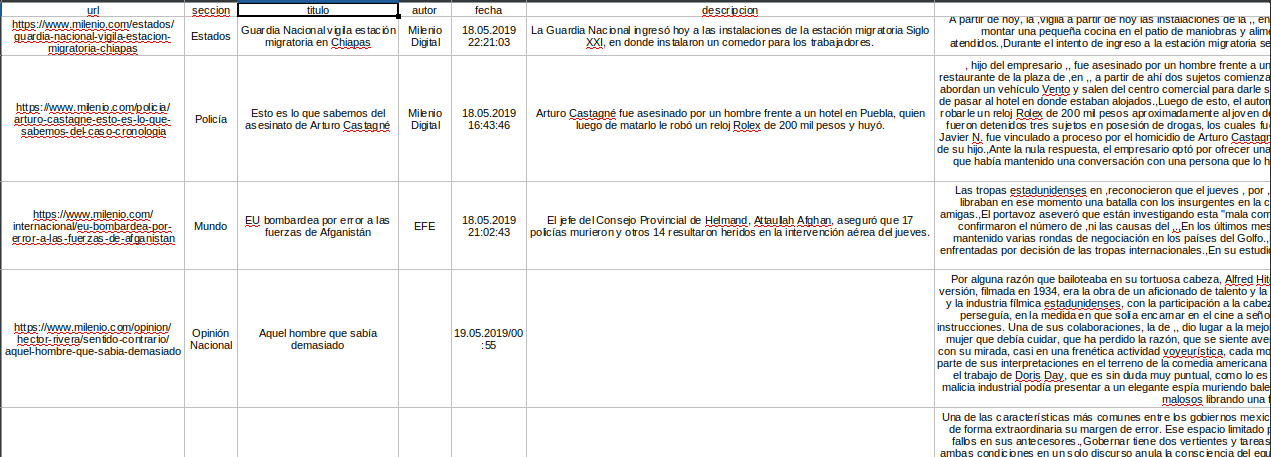
\includegraphics[scale=.3]{imagenes/Capitulo5/9}
  \caption{Resultados obtenidos de la extracción del sitio web almacenado en un archivo CSV.}
  \label{fig:nueve}
\end{figure}

%-----------------------------------------------------------------------------------------%
\subsection{Consideraciones}
\begin{itemize}
  \item Se debe tener conocimiento de XML para poder realizar las etiquetas que extraen información de la cada sitio web
  \item Cuando la noticia consta de un video, no se obtiene ninguna información adicional de la noticia
  \item Se debe tomar en cuenta que las secciones no están homologadas, es decir a pesar de que de la misma página existan varias secciones 
en la cual una noticia puede ser clasificada.
  \item La distribución de la información de una noticia varia dependiendo a la sección y sitio web.
  \item Se acotó el periodo de búsqueda de noticias ya que algunos sitios web muestran las noticias más recientes.
\end{itemize}

%-----------------------------------------------------------------------------------------%
\subsection{Conclusiones}
%Conclusiones
%A pesar de extraer la mayoría de etiquetas requeridas, existen algunos datos que se encuentran en una sola etiqueta.
El 75\% de los sitios web seleccionados contienen las secciones definidas. sin embargo
los sitios web de foros de noticias (Aristegui Noticias, SDP Noticias y Sopitas) tienen muy pocas secciones. A demás 
se logró desarrollar un recolector de noticias que permite extraer el contenido deseado de cada portal como las secciones de los artículos y las URLs que dirigen a noticias asociadas.

%Escribirlo de manera más precisa

%-----------------------------------------------------------------------------------------%
\section{Trabajo a futuro}
\begin{itemize}
  \item Una vez que se obtuvo la extracción de las noticias, analizarán para su integración al corpus
  \item Corregir las reglas para la extracción de la información de los sitios web, y así evitar extraer información con código HTML
  \item Agregar reglas para cada etiqueta, de manera tal manera que se obtenga la información necesaria
  \item Realizar el clasificador de noticias aplicando las técnicas de clasificación previamente definidas
\end{itemize}


